\chapter{CONTRASTOS DE LA KHI-QUADRAT}\label{capitol-khi-quadrat}

\section{Introducci\'{o}}

Amb el nom de proves khi-quadrat es coneix una varietat de tests
estad\'{i}stics que fan refer\`{e}ncia a problemes diferents
per\`{o} tenen els seg\"{u}ents trets en com\'{u}:

\begin{itemize}
\item  Les mostres corresponen a dades categ\`{o}riques, \emph{directament o
per categoritzaci\'{o} d'una variable num\`{e}rica}, \'{e}s a dir
es mesura si un individu pertany a un element d'una partici\'{o}
$A_1,A_2,...,A_k$ de l'espai mostral.

\item  L'estad\'{i}stic de test t\'{e} una estructura comuna:
\[
\sum_i\frac{\left( O_i-E_i\right) ^2}{E_i}
\]
essent

\begin{itemize}
\item  $O_i$ el nombre de valors observats en una determinada categoria i

\item  $E_{i\text{ }}el$ nombre de valors esperats en aquella categoria en
cas que la hip\`{o}tesi nul:la fos certa.
\end{itemize}

\item  L'estad\'{i}stic de test segueix una distribuci\'{o} $\chi ^2$
\end{itemize}

Considerem tres grans grups de proves

\begin{enumerate}
\item  Proves d'ajustatge (``goodness of fit'')\ d'unes dades a una
distribuci\'{o}

\begin{enumerate}
\item  Tots els par\`{a}metres de la distribuci\'{o} s\'{o}n coneguts

\item  Alguns par\`{a}metres de la distribuci\'{o} s\'{o}n desconeguts
\end{enumerate}

\item  Proves d'independ\`{e}ncia

\item  Proves d'homogene\"{i}tat
\end{enumerate}

\section{Proves $\chi ^2$ de bondat d'ajustatge}
\subsection{Hip\`{o}tesis simples}
Donada una m.a.s. $X_1,X_{2,}...,X_n$ d'una variable $X\,\,$volem
contrastar la hip\`{o}tesi de que la variable es distribueix
segons una certa distribuci\'{o} completament especificada
$F_{\theta _0}$.
\begin{eqnarray*}
H_0 &:&X\sim F_{\theta _0} \\
H_1 &:&X\nsim F_{\theta _0}.
\end{eqnarray*}
Sigui $R$ el recorregut de la distribuci\'{o} poblacional.
Considerem una partici\'{o} de $R$ en $k$ subconjunts disjunts
$R_1,R_2,...,R_k.$ Aix\`{o}
genera una partici\'{o} en $k$ esdeveniments $A_1,A_2,...,A_k$%
\[
A_i=X\in R_i,\text{ \quad }i=1,...,k
\]
de forma que la variable $k$-dimensional $(n_1,...,n_k)\;que$
compta el
nombre d'observacions de la mostra en cada un dels subconjunts $%
R_1,R_2,...,R_k$ t\'{e} distribuci\'{o} multinomial
\[
Y\sim M(n;p_1,...,p_k).
\]
Aquest plantejament transforma el contrast inicial referit a la
distribuci\'{o} d'$X$ en un contrast sobre les probabilitats $p_1,...,p_k$%
\begin{eqnarray}
H_0 &:&P(A_i)=p_i^0,\quad \left( =\int_{R_i}dF_{\theta _0}(x)\right) \\
H_1 &:&P(A_i)=p_i\neq p_i^0. \label{test-ajust-1}
\end{eqnarray}
Observem que no es contrasta el fet que $Y$ tingui distribuci\'{o}
multinomial sino si les probabilitats es determinen o no per la
distribuci\'{o} proposat per la hip\`{o}tesi nul$.$la.

\subsection{Estad\'{i}stic de test per a les proves $\chi ^2$ d'ajustage}

A\ comen\c{c}aments de segle l'estad\'{i}stic Karl Pearson va
proposar de fer servir, per a aquest test, l'estad\'{i}stic
seg\"{u}ent. Considerant la partici\'{o} anterior diguem
$n_i,i=1,...,k$ el nombre d'individus observats en la
partici\'{o} $A_i.$ Si la hip\`{o}tesi nula fos certa esperariem
que el nombre d'individus en A$_i$ fos: $E_i=n\cdot
P_{H_0}(A_i)=np_i^0.$ Una mesura raonable de la discrep\`{a}ncia
entre el que s'observa i el que postula la hip\`{o}tesi nula ve
donat per:
\[
D^2=\sum_{i=1}^k\frac{\left( n_i-np_i^0\right) ^2}{np_i^0}.
\]
L'interes especial que t\'{e} aquest estad\'{i}stic \'{e}s que, a
difer\`{e}ncia d'altres que podr\'{i}em concebre, \emph{es coneix
la seva distribuci\'{o} asimpt\`{o}tica sota la hip\`{o}tesi
nula} de forma que es possible fer-lo servir per construir una
regi\'{o} cr\'{i}tica per a les hip\`{o}tesis
\[
H_0:P(A_i)=p_i^0,\quad H_1:P(A_i)\neq p_i^0.
\]

El resultat principal d'aquesta secci\'{o}, que permet construir
el test, \'{e}s el teorema seg\"{u}ent, degut a K. Pearson:

\begin{theorem}
\label{teorema-khi2-1}
Sota les condicions descrites m\'{e}s amunt si les probabilitats $%
p_1^0,...,p_k^0$ s\'{o}n nombres coneguts aleshores
l'estad\'{i}stic
\[
D^2=\sum_{i=1}^k\frac{\left( n_i-np_i^0\right) ^2}{np_i^0}.
\]
t\'{e} distribuci\'{o} asimpt\`{o}tica $\chi ^2$ amb $k-1$ graus
de llibertat
\[
D^2\stackrel{\pounds }{\stackunder{n\rightarrow \infty
}{\rightarrow }}\chi _{k-1}^2
\]
\end{theorem}
Podeu veure la demostraci\'{o} d'aquest teorema a Martinez i alt.
(\cite{Martinez-93}).

En base al teorema anterior podem establir el seg\"{u}ent test
\begin{definition}\textbf{Test de bondat
d'ajustatge} Sigui $X\sim F_\theta ,\left( \theta \in \Theta
\subset \Real^m\right)$ i siguin
$R:\text{Rec}(X)=\biguplus_{i=1}^kR_i$ i $A_i=\left\{ X\in
R_i\right\} ,P(A_i)=p_i $. Sigui $Y=\left( n_1,...,n_k\right)
,\text{ }n_i=\#A_i$ que verifica $Y\sim M\left( n;{\bf
p}=(p_1,...,p_k)\right)$. Aleshores, per contrastar la hip\`{o}tesis:
\beqa
H_0:&& \ X\sim F_{\theta _0}^0\Leftrightarrow {\bf
p}=(p_1^0,...,p_k^0)\\
H_1:&& \ {\bf p}\neq (p_1^0,...,p_k^0),
\eeqa
el test consistent en rebutjar $H_0$ si $D^2\geq \chi
_{k-1,1-\alpha }^2$, on
$$
\begin{array}{l}
D^2=\sum_{i=1}^k\dfrac{\left( n_i-np_i^0\right) ^2}{np_i^0} \\
D^2\stackrel{\pounds }{\stackunder{n\rightarrow \infty
}{\rightarrow }}\chi _{k-1}^2, \label{Ajust-khi2-1}
\end{array}
$$
\'{e}s un test asimpt\`{o}tic de nivell $\alpha$.
\end{definition}

Aquest resultat estableix que una regi\'{o} cr\'{i}tica per al
test \ref{test-ajust-1} tindr\`{a} la forma
\[
W=\left\{ D^2\geq \chi _{k-1,1-\alpha }^2\right\} ,
\]
on $\chi _{k-1,1-\alpha }^2$ \'{e}s el quantil $1-\alpha $ d'una
distribuci\'{o} $\chi ^2$ amb $k-1$ graus de llibertat.

\subsubsection{Observacions}
Hi ha alguns punts que cal tenir en compte per a que les
conclusions derivades d'aquest test siguin fiables.
\begin{itemize}
\item Es tracta d'un test asimpt\`{o}tic i per tant \'{e}s v\`{a}lid per
mostres de mida gran. En la pr\`{a}ctica se sol requerir que
$np_i^0\geq 5,\quad \forall i=1,2,...,k$.
\item El test no discrimina entre distribucions que assignen la
mateixa probabilitat als conjunts $A_i$. Per exemple, com a cas
extrem, si agaf\'{e}ssim $k=2$ i $A_1=[X\leq E(X)]$, $A_2=[X \geq
E(X)]$ totes les distribucions sim\`{e}triques assignarien la mateixa
probabilitat a cada categoria. En conseq\"{u}\`{e}ncia conv\'{e} agafar
$k\geq 5$ sempre que es pugui. Com aix\`{o} implicar\`{a} necess\`{a}riament
alguna $p_i^0\leq 1/5$ vol dir que com a m\'{\i}nim cal $n\geq 25$.
\end{itemize}

\begin{example}
Una companyia afirma que el nombre diari d'accidents laborals
segueix una distribuci\'{o} de Poisson de par\`{a}metre
$\lambda=2$. Un estudi, basat en els accidents produ\"{\i}ts
durant 200 dies d\'{o}na el resultat seg\"{u}ents: \vskip
0.5cm\begin{center}
\begin{tabular}{|l|c|c|c|c|c|c|c|c|}
\hline
  N� d'accidents & 0 & 1 & 2 & 3 & 4 & 5 & 6 & 7 \\
  Dies & 22 & 53 & 58 & 39 & 20 & 5 & 2 & 1 \\ \hline
\end{tabular}
\end{center}
\vskip 0.5cm Per contrastar l'ajustatge a una distribuci\'{o} de
Poisson hem de calcular les probabilitats
$$
p_i^0=P_{\lambda=2}[X=i]=e^{-\lambda}\frac{\lambda^i}{i!},\quad
i=1,...,7.
$$
Les freq\"{u}\`{e}ncies esperades seran $np_i^0=200p_i^0$. Quan
$i=6, 7$ els valors s\'{o}n massa petits de forma que s'agrupen
els valors en una \'{u}nica categoria ``$i\geq 5$''.

\begin{center}\vskip 0.5cm
\begin{tabular}{||l|c|c|c|c|c|c|c||c||}
\hline\hline
 $x_i$   &   0   &   1   &   2   &   3   &   4   &   $\geq 5$&$\Sigma$\\ \hline
$n_i$ &   22  &   53&   58  &   39  &   20  &   8 & 200\\\hline
$p_i^0$ &   0.135   &   0.271   &   0.271 &   0.180   &   0.090
&0.053& 1\\\hline
 $np_i^0$ &   27.067  &   54.134  &54.134  &   36.089  &   18.045  &   10.531 & 200 \\\hline
 $\ds\frac{(np_i^0-n_i)^2}{np_i^0}$ &   0.9486  & 0.0238 &   0.2761  &   0.2347  &
 0.2119  &   0.6081 & \textbf{2.303}\\ \hline\hline
\end{tabular}
\vskip 0.5cm \end{center}

El valor de l'estad\'{\i}stic de test \'{e}s doncs 2.303. El
$p-valor$ corresponent, \'{e}s a dir, $P(\chi^2_{6-1}\geq 2.303$
\'{e}s de 0.80588 i per tant no podem rebutjar la hip\`{o}tesi de
que les dades segueixen una distribuci\'{o} de Poisson de
par\`{a}metre $\lambda=2$. Una altra forma de prendre la mateixa
decisi\'{o} \'{e}s observant que el percentil 0.95 d'aquesta
distribuci\'{o} \'{e}s $\chi^2_{5,0.95}=11.07$ d'on, at\`{e}s
que  $2.303 < \chi^2_{5,0.95}$ veiem que no podem rebutjar $H_0$.
\end{example}

\begin{example}\label{model-genetic-1}
Un cert model gen\`{e}tic per a unes plantes les flors de les
quals poden ser blanques roses o vermelles afirma que la
proporci\'{o} amb qu\`{e} han d'apar\`{e}ixer \'{e}s de $1:2:1$.
En un estudi es van obtenir 113 flors blanques, 242 roses i 112
de vermelles. Concorden les observacions amb el model?
Constru\"{\i}m la taula dels c\`{a}lculs obtenim: \vskip 0.5cm

\vskip 0.5cm\begin{center}
\begin{tabular}{||l|c|c|c||c||}
\hline\hline
 $A_i$   &  Blanca    &   Rosa   &   Vermelles  &$\Sigma$\\ \hline
$n_i$ &   112  &   242&   112  &   467\\ \hline $p_i^0$ & 0.25
&0.5   &   0.25 &    1\\\hline
 $np_i^0$ &   116.7  & 233 & 116.7  & 467 \\\hline
 $\ds\frac{(np_i^0-n_i)^2}{np_i^0}$ &   0.117  & 0.348 &  0.193  &
 \textbf{0.657}\\ \hline\hline
\end{tabular}
\end{center} \vskip 0.5cm

El valor cr\'{\i}tic \'{e}s el percentil d'una distribuci\'{o}
khi-quadrat amb dos graus de llibertat, $\chi^2_{2,0.95}=5.99$
d'on, at\`{e}s que $0.657 < \chi^2_{2,0.95}$ veiem que no podem
rebutjar $H_0$.
\end{example}

Observem que el primer exemple \'{e}s una variable num\`{e}rica que s'ha
categoritzat mentre que el segon fa refer\`{e}ncia directament a una
distribuci\'{o} multinomial.

\subsection{Hip\`{o}tesis compostes}
El test d'ajustatge que hem discutit en la secci\'{o} anterior es
correspon amb una situaci\'{o} poc usual. En la pr\`{a}ctica, el que ens
interessar\`{a} \'{e}s decidir si les dades s'ajusten a una determinada
fam\'{\i}lia de distribucions. Per exemple, abans de aplicar un test on
se suposa que les dades segueixen una llei Normal s'ha de
verificar fins quin punt \'{e}s v\`{a}lida aquesta suposici\'{o}.

En aquest cas ens trobem en una situaci\'{o} an\`{a}loga a l'anterior,
excepte pel fet que la distribuci\'{o} no est\`{a} completament
especificada sin\'{o} que dep\`{e}n d'un par\`{a}metre $m$--dimensional.
\beqa
X&\sim& F_\theta ,\left( \theta \in \Theta \subset \Real ^m\right)  \\
R&=&\text{Rec}(X)=\biguplus_{i=1}^kR_i ,\quad A_i=\left\{ X\in
R_i\right\} ,P(A_i)=p_i(\theta)\Longrightarrow\\
Y&=&\left( n_1,...,n_k\right) ,\text{ }n_i=\#A_i \quad Y\sim
M\left( n;{\bf p}=\left(p_1(\theta),...,p_k(\theta)\right)\right).
\eeqa

Una primera idea que se'ns podria oc\'{o}rrer per afrontar aquest
problema seria estimar $\theta$ mitjan\c{c}ant un estimador $\hat
\theta$ i substituir $p_i^0$ per $p_i(\hat\theta)$ en
(\ref{Ajust-khi2-1}). Aix\`{o} no seria mala idea si l'estimaci\'{o} es
bases en una mostra diferent de la que es fa servir per fer
l'ajustatge.

Ara b\'{e}, aquest no \'{e}s el cas aqu\'{\i}. Si fem servir la
mostra per estimar els par\`{a}metres i despr\'{e}s fem l'ajust estem
``for\c{c}ant la mostra'' a seleccionar la distribuci\'{o} poblacional
per tal que s'ajusti b\'{e} a la mostra a trav\'{e}s de l'estimaci\'{o} dels
par\`{a}metres (estem fent un ajust condicionat). Per compensar-ho
mirarem de ser ```m\'{e}s exigents" a l'hora de jutjar si les
freq\"{u}\`{e}ncies observades es corresponen amb les esperades, i aix\`{o}
es reflectir\`{a} en que enlloc de basar-nos en una distribuci\'{o}
$\chi^2$ amb $k-1$ graus de llibertat ho farem en una amb $k-1-m$
graus de llibertat, on $m$ representar\`{a} el nombre de par\`{a}metres
que ens ha calgut estimar. Aquest resultat s'expressa en el teorema seg\"{u}ent:

\begin{theorem}\label{teorema-khi2-2}
Sota les condicions del teorema \ref{teorema-khi2-1} suposem que les probabilitats
$p_1,...,p_k$ depenen de par\`{a}metres desconeguts $\theta=\theta_1,...,\theta_m$.
Siguin $\hat\theta=\hat\theta_1,...,\hat\theta_m$ les estimacions del m\`{a}xim de versemblan\c{c}a dels par\`{a}metres $\theta$ i suposem que es verifiquen les seg\"{u}ents condicions de regularitat
\begin{enumerate}
\item Les derivades parcials $\frac {\partial p_i}{\partial \theta_j}$, $\frac {\partial^2 p_i}{\partial \theta_i \partial \theta_j}$ existeixen i s\'{o}n cont\'{\i}nues.
\item La matriu jacobiana $\frac {\partial p_i}{\partial \theta_j}$ $i=1,..,k$, $j=1,..m$ t\'{e} rang $m$.
\end{enumerate}
aleshores l'estad\'{i}stic
\[
D^2=\sum_{i=1}^k\dfrac{\left( n_i-np_i(\hat{\theta})\right) ^2}{np_i(%
\hat{\theta})}
\]
verifica
$$
D^2\stackrel{\pounds }{\stackunder{n\rightarrow \infty }{\rightarrow }}\chi
_{k-1-\dim (\Theta )}^2
$$
\'{e}s a dir t\'{e} distribuci\'{o} asimpt\`{o}tica $\chi ^2$ amb $k-1-\dim (\Theta )$ graus
de llibertat
\end{theorem}

Podem procedir de forma an\`{a}loga al cas de probabilitats conegudes per establir el test seg\"{u}ent:
\begin{definition}\textbf{Test de bondat d'ajustatge quan cal estimar par\`{a}metres}
Siguin:
\begin{eqnarray*}
X&\sim& F_\theta ,\left( \theta \in \Theta \subset \Re ^m\right) \quad
R:\text{Rec}(X)=\biguplus_{i=1}^kR_i \\
A_i&=&\left\{ X\in R_i\right\} ,P(A_i)=p_i(\theta) \\
Y&=&\left( n_1,...,n_k\right) ,\text{ }n_i=\#A_i, \quad
Y\sim M\left( n;{\bf p}=(p_1(\theta),...,p_k(\theta))\right).
\end{eqnarray*}
Aleshores, per contrastar la hip\`{o}tesis:
\beqa
H_0:&& X\sim F_\theta ^0\Leftrightarrow {\bf p}=\left( p_1(\theta ),...,p_k(\theta )\right)\\
H_1:&& {\bf p}\neq \left( p_1(\theta ),...,p_k(\theta )\right)
\eeqa
el test consistent en rebutjar $H_0$ si
$ D^2\geq \chi _{k-1-\dim (\Theta ),1-\alpha }^2$, on
\beqa
D^2&=&\sum_{i=1}^k\dfrac{\left( n_i-np_i(\hat{\theta})\right) ^2}{np_i(
\hat{\theta})} \\
D^2&&\stackrel{\pounds }{\stackunder{n\rightarrow \infty }{\rightarrow }}\chi
_{k-1-\dim (\Theta )}^2
\eeqa
\'{e}s un test asimpt\`{o}tic de nivell $\alpha$.
\end{definition}

Aquest resultat estableix que una regi\'{o} cr\'{i}tica per al
test \ref{test-ajust-1} tindr\`{a} la forma
\[
W=\left\{ D^2\geq \chi _{k-1-\dim (\Theta),1-\alpha }^2\right\} ,
\]
on $\chi _{k-1,1-\alpha }^2$ \'{e}s el quantil $1-\alpha $ d'una
distribuci\'{o} $\chi ^2$ amb $k-1-\dim (\Theta)$ graus de llibertat.


\begin{example}
En l'exemple (\ref{model-genetic-1}), quan hem ajustat unes dades a unes proporcions del tipus ``1:2:1" o ``9:3:3:1" est\`{a}vem suposant dues coses:
\begin{itemize}
\item Un model gen\`{e}tic (que no tenim per qu\`{e} con\`{e}ixer)
\item Unes probabilitats fixades.
\end{itemize}
Aix\`{o} ho hem sintetitzat en un vector num\`{e}ric $(p_1^0,...,p_k^0)$. Per exemple, en (\ref{model-genetic-1}) la proporci\'{o} ``1:2:1" ve de suposar:
\begin{itemize}
\item Com a model: $p^2,\ 2p(1-p),\ q^2$,
\item Com probabilitats: $p=\frac 12$.
\end{itemize}
Sovint ens interessa ajustar nom\'{e}s el model, \'{e}s a dir decidir si p.ex. el model $p^2,\ 2p(1-p),\ q^2$ descriu b\'{e} les dades observades per alguna $p\in (0,1)$. En aquest cas abans de comparar els observats $n_i$ amb els esperats $p_i$ haurem d'estimar els valors dels $p_i$.

Sota la suposici\'{o} d'un model multinomial
\beqa
Y \sim M(n,{\bold p(\theta)}, \quad &&\theta=p,\\
&& p_1(\theta)=p^2,\ p_2(\theta)=2p(1-p),\
p_3(\theta)=(1-p)^2
%=1-(p_1(\theta)-p_2(\theta))
\eeqa
la versemblan\c{c}a del model \'{e}s:
$$
L\left (n_1,...,n_k;{\bold p(\theta)}\right)\propto
(p^2)^{n_1}\cdot (2p(1-p))^{n_2}\cdot(q^2)^{n_3}.
$$
Una aplicaci\'{o}
rutin\`{a}ria del m\`{e}tode del m\`{a}xim de versemblan\c{c}a
d\'{o}na com estimador del m\`{a}xim de versemblan\c{c}a de $p$:
$$
\hat p_{MV}=\frac{2n_1+n_2}{2n_1+2n_2+2n_3}.
$$
Suposem ara que tenim unes dades gen\`{e}tiques corresponents al grup sanguini M--N en una poblaci\'{o} de 6129 individus, indis navajos,  que s\'{o}n les seg\"{u}ents:

\vskip 0.5cm\begin{center}
\begin{tabular}{|l|c|c|c||}
\hline
  Grup & M & M--N & N \\
  Individus & 1787 & 3039 & 1303 \\ \hline
\end{tabular}
\end{center}\vskip 0.5cm

L'estimador del m\`{a}xim de versemblan\c{c}a calculat sobre les dades de l'exemple \'{e}s:
$$
\hat p_{MV}=\frac{2\cdot 1787+3039}{2\cdot 1787+2\cdot 3039+2\cdot 1303}=0.539
$$
d'on la taula amb els valors observats i esperats per fer el test d'ajust \'{e}s:

\vskip 0.5cm\begin{center}
\begin{tabular}{||c|c|c|c||c||}
\hline\hline
    &  M&   M--N&   N&$\Sigma$\\ \hline
$n_i$ &   1787  &   3039&   1303  &   6129\\ \hline
$p_i\left(\hat p_{MV}\right)$ & 0.539& 2$\cdot$ 0.539$\cdot$ 0.461   &   0.461&
1\\\hline
 $np_i\left(\hat p_{MV}\right)$ &   1784  & 3046 & 1299.8  & 6129 \\\hline
 $\ds \frac{\left (np_i\left(\hat p_{MV}\right)-n_i\right)^2}{np_i\left(\hat p_{MV}\right)}$ &   0.0067  & 0.0166 &  0.0078  &
 \textbf{0.0311}\\ \hline\hline
\end{tabular}
\end{center}\vskip 0.5cm

 El valor cr\'{\i}tic \'{e}s el percentil d'una
distribuci\'{o} khi-quadrat amb dos \textbf{menys un }graus de
llibertat, $\chi^2_{1,0.95}=3.841$ d'on, at\`{e}s que $0.0311 <
\chi^2_{1,0.95}$ veiem que no podem rebutjar $H_0$.
\end{example}

\begin{example}
En un estudi sobre biling\"{u}isme es va aplicar una prova sobre una
mostra de 211 alumnes i es van obtenir 211 puntuacions que, un
cop tabulades eren les seg\"{u}ents:

\begin{center}
\small
\begin{tabular}{|l|c|c|c|c|c|c|c||}
\hline
  Puntuaci\'{o} & $(\leq 55]$ &$(55-60]$&$(60-65]$ &$(65-70]$ &$(70-75]$&$(75-80]$&$(80-85]$\\\hline
  Freq\"{u}\`{e}ncia & 4 & 17 & 45 & 67 & 53 & 15 & 10 \\ \hline
\end{tabular}
\normalsize
\end{center}

Podem acceptar la hip\`{o}tesi de que la puntuaci\'{o} segueix una
distribuci\'{o} normal?

Fixem-nos que aqu\'{\i} no ens interessa m\'{e}s que el fet que sigui
normal, no, una normal en concret. Es a dir tenim:
\beqa
H_0:&& \ X\sim N(\mu,\sigma)\\
H_1:&& \ X \nsim N(\mu,\sigma).
\eeqa
En primer lloc estimem els par\`{a}metres els par\`{a}metres:
\beqa
\hat \mu & =& \overline{X}=68.52\\
\hat \sigma^2 & =&S^2=6.44
\eeqa
Cada categoria $A_i$ \'{e}s un interval del recorregut de la
variable: $A_1=X\in (-\infty,55]$, $A_2=X\in (55, 60]\ \dots$, de
manera que si $A_i=(a,b]$, les probabilitats $p_i=P(A_i)$ es
calcularan, si suposem que $Y$ representa una variable amb
distribuci\'{o} normal de mitjana $\hat \mu=\overline{x}$ i desviaci\'{o}
t\'{\i}pica $\hat \sigma=s^2$:
\beqa
p_i=p_i(\overline{x},s^2)&=&P_{\overline{x},s^2}(X\in
A_i)=F_Y(b)-F_Y(a)\\
&=&\Phi\left (\frac{b-\overline{x}}{s}\right)- \Phi\left
(\frac{a-\overline{x}}{s}\right),
\eeqa
on $\Phi$ \'{e}s la funci\'{o} de distribuci\'{o} de probabilitat d'una
variable $N(0,1)$.

Si calculem les probabilitats en aquests intervals i constru\"{\i}m la
taula obtenim:

\begin{center}
\small
\begin{tabular}{|l|c|c|c|c|c|c|c||}
\hline
 Puntuaci\'{o}  & $(\leq 55]$ &$(55-60]$&$(60-65]$ &$(65-70]$ &$(70-75]$&$(75-80]$&$(\geq 80)$ \\\hline
 $n_i$ & 4 & 17 & 45 & 67 & 53 & 15 & 10 \\ \hline
$p_i(\overline{x},s^2)$ & 0.01786&0.07556 & 0.19774 & 0.29979 &
0.2528 & 0.11871 & 0.03654 \\ \hline
$n\cdot
p_i(\overline{x},s^2)$ & 3.77 & 15.94 & 41.72 & 63.26 &
53.34 & 25.05 & 7.92 \\
\hline
\end{tabular}
\normalsize
\end{center}

Abans de calcular el valor de l'estad\'{\i}stic de test cal refondre
les dues primeres columnes ja que la freq\"{u}\`{e}ncia esperada \'{e}s
inferior a 5. La taula final queda:

\begin{center}
\small
\begin{tabular}{|l|c|c|c|c|c|c||}
\hline
 Puntuaci\'{o}  & $(\leq 60]$&$(60-65]$ &$(65-70]$ &$(70-75]$&$(75-80]$&$(\geq 80)$ \\\hline
 $n_i$ & 4 + 17 & 45 & 67 & 53 & 15 & 10 \\ \hline
$n\cdot p_i(\overline{x},s^2)$ & 3.77 + 15.94 & 41.72 & 63.26 &
53.34 & 25.05 & 7.92 \\
\hline
\end{tabular}
\normalsize
\end{center}

L'estad\'{\i}stic de test, $D^2$ val aqu\'{\i}: 5.144. Com hem estimat 2
par\`{a}metres i la taula final t\'{e} 6 columnes obtindrem el valor
cr\'{\i}tic d'una $\chi^2$ amb $6-2-1$ grau de llibertat. En concret:
rebutjarem $H_0$ si $D^2 > \chi^2_{(3,0.05)}$. Com aix\`{o} no \'{e}s aix\'{\i}
no podem rebutjar $H_0$.
\end{example}

\section{Proves d'independ\`{e}ncia en taules de conting\`{e}ncia}

Sigui $\Omega$ una poblaci\'{o} que admet dues descomposicions diferents en esdeveniments excloents. Per exemple una descomposici\'{o} pot fer-se pel sexe (homes/dones) i l'altre pel tabaquisme (fumadors/no fumadors).
$$
\Omega=A_1 \biguplus \dots \biguplus A_k= B_1 \biguplus \dots \biguplus B_r,
$$
on el signe $\biguplus$ indica uni\'{o} disjunta.
Suposem que es realitzen n observacions o proves independents de manera que $n_ij$ representa la freq\"{u}\`{e}ncia amb que es presenta l'esdeveniment $A_i\bigcap B_j$. Podem disposar les observacions en una taula creuada o de conting\`{e}ncia d'$r$ files per $k$ columnes:
$$
\begin{tabular}{l|lll|l}
& $A_1$ & $\cdots $ & $A_k$ &  \\ \hline
B$_1$ & n$_{11}$ & $\cdots $ & n$_{1k}$ & n$_{1.}$ \\
$\vdots $ & $\vdots $ & $\ddots $ & $\vdots $ &  \\
B$_r$ & n$_{r1}$ & $\cdots $ & n$_{kr}$ & n$_{r.}$ \\ \hline
& n$_{.1}$ &  & n$_{.k}$ & n
\end{tabular}
$$
on $n_{i.}=\sum_{i=1}^k n_{ij}$ \'{e}s la freq\"{u}\`{e}ncia de l'esdeveniment $A_i$ i
$n_{.j}=\sum_{i=1}^r n_{ij}$ \'{e}s la freq\"{u}\`{e}ncia de l'esdeveniment $B_j$.

Suposem que volem contrastar la hip\`{o}tesi de que les dues particions s\'{o}n independents, \'{e}s a dir:
\beqa
H_0:&& A_i \text{ \'{e}s estoc\`{a}sticament independent d'}B_j, \Longleftrightarrow\\
&&P(A_i\bigcap B_j)=P(A_i)\times P(B_j),\  i=1,\dots k,\ j=1,\dots r.
\eeqa
Si indiquem $p_{ij}=P(A_i\bigcap B_j)$ i introdu\"{\i}m els par\`{a}metres
$$
p_{1.},\dots,p_{r.},\quad \sum_{i=1}^rp_{i.}=1,\quad
p_{.1},\dots,p_{.k},\quad \sum_{j=1}^kp_{.j}=1,
$$
la hip\`{o}tesi nul.la s'expressar\`{a} com:
$$
p_{ij}=p_{i.}\times p_{.j}.
$$
\'{E}s f\`{a}cil veure que, en aquest cas, els estimadors del m\`{a}xim de versemblan\c{c}a de les probabilitats s\'{o}n les freq\"{u}\`{e}ncies relatives:
$$
\hat p_{i.}=\frac{n_{i.}}n,\quad , \hat p_{.j}=\frac{n_{.j}}n,
$$
i la freq\"{u}\`{e}ncia esperada de l'esdeveniment $A_i\bigcap B_j$ sota $H_0$ ser\`{a}
$$
n \hat p_{i.}\times \hat p_{.j}= n\times \frac{n_{i.}}n,\times \frac{n_{.j}}n=
\frac{n_{i.}\times n_{.j}}n.
$$
Aplicant el teorema ~\ref{teorema-khi2-2} tenim que l'estad\'{\i}stic:
$$
D^2=\sum_{i=1}^k\sum_{j=1}^r\dfrac{\left( n_{ij}-\dfrac{%
n_{i.}}n\dfrac{n_{.j}}nn\right) ^2}{\dfrac{n_{i.}}n\dfrac{n_{.j}}nn}
$$
verifica
$$
D^2\stackrel{\pounds }{\stackunder{n\rightarrow \infty }{\rightarrow }}\chi
_{(r-1)(k-1))}^2.
$$
Com a conseq\"{u}\`{e}ncia de l'anterior el test d'independ\`{e}ncia per a la hip\`{o}tesi
\beqa
H_0:&& A_i \text{ \'{e}s estoc\`{a}sticament independent d'}B_j, \Longleftrightarrow\\
&&P(A_i\bigcap B_j)=P(A_i)\times P(B_j),\  i=1,\dots k,\ j=1,\dots r,\ \Longleftrightarrow\\
&&p_{ij}=p_{i.}\times p_{.j}.,
\eeqa
consistir\`{a} en calcular
$$
D^2=\sum_{i=1}^k\sum_{j=1}^r\dfrac{\left( n_{ij}-\dfrac{%
n_{i.}}n\dfrac{n_{.j}}nn\right) ^2}{\dfrac{n_{i.}}n\dfrac{n_{.j}}nn}
$$
i rebutjar $H_0$ si $D^2\geq \chi _{(k-1)(r-1),1-\alpha}^2$.

\begin{example}
En un estudi de mercat s'est\`{a} intentant determinar si hi ha alguna relaci\'{o} entre les prefer\`{e}ncies d'un grup de consumidors per un tipus de vehicle i el nivell cultural d'aquests. Es pregunta a 300 persones entre 20 i 50 anys quin vehicle tenen i es classifiquen en "CAP", "MOTOS", "COTXES NORMALS" i "COTXES POTENTS".
El nivell cultural es determina per si han cursat estudis "ELEMENTALS",  "DE GRAU MIG" o "SUPERIORS". Qu\`{e} podrem dir a partir de les dades seg\"{u}ents ?.

\begin{center}
\begin{tabular}{||c|c|c|c|c|c||}
 \hline \hline
 & CAP & MOTOS & C. NORMAL & C.POTENT & TOTAL \\ \hline
Elementals & 31 & 49 & 18 & 12 & 110 \\\hline
Nivell mig & 11 & 59 & 26 & 25 & 121 \\\hline
Superiors & 12 & 51 & 31 & 36 & 130 \\\hline
TOTAL & 54 & 159 & 75 & 73 & 361 \\ \hline \hline
\end{tabular}
\end{center}
La taula amb els valors esperats \'{e}s:
\begin{center}
\begin{tabular}{||c|c|c|c|c|c||}
 \hline \hline
 & CAP & MOTOS & C. NORMAL & C.POTENT & TOTAL \\ \hline
Elementals & 16.5 & 48.4 & 22.9 & 22.2 & 110 \\\hline
Nivell mig & 18.1 & 53.3 & 25.1 & 24.5 & 121 \\\hline
Superiors & 19.4 & 57.3 & 27.0 & 26.3 & 130 \\\hline
TOTAL & 54 & 159 & 75 & 73 & 361 \\ \hline \hline
\end{tabular}
\end{center}
El valor de l'estad\'{\i}stica de test $D$ calculat sobre aquestes dades \'{e}s de: 29.76.
El valor de la taula de $\chi$--quadrat amb $(4-1)\cdot(3-1) = 6$ graus de llibertat i $0.05$ de nivell de significaci\'{o} \'{e}s de : 12.59, at\`{e}s que
$$
D^2 29.76 \geq 12.59 =\chi _{(3-1)(4-1),1-0.05}^2
$$
rebutgem la hip\`{o}tesi d'independ\`{e}ncia, \'{e}s a dir s\'{\i} sembla haver-hi relaci\'{o} entre el nivell d'estudis i el tipus de vehicle.

%El gr\`{a}fic de la figura \ref{testindep} confirma la conclusi\'{o} ja que mostra una certa %tend\`{e}ncia a tenir un vehicle m\'{e}s potent amb un nivell d'estudis m\'{e}s baix.
%
%\begin{figure}[ht]
%\begin{center}
%\includegraphics{TestIndep.eps}
%\end{center}
%\caption{Diagrama de barres m\'{u}ltiples que mostra com es
%distribueixen els tipus de vehicles segons el nivell d'estudis
%ra\c{c}a}\label{testindep}
%\end{figure}

\end{example}

\section{Proves d'homogene\"{\i}tat}
Suposem que tenim un a mateixa partici\'{o}
$$
\Omega=A_1 \biguplus \dots \biguplus A_k,
$$
en $R$ poblacions,
$$
\begin{tabular}{l|lll|l}
& $A_1$ & $\cdots $ & $A_k$ &  \\ \hline
I & n$_{11}$ & $\cdots $ & n$_{1k}$ & n$_1$ \\
$\vdots $ & $\vdots $ & $\ddots $ & $\vdots $ &  \\
$R$ & n$_{r1}$ & $\cdots $ & n$_{kr}$ & n$_r$ \\ \hline
& n$_{.1}$ &  & n$_{.k}$ & n
\end{tabular}
$$
i volem contrastar la hip\`{o}tesis
$$
\begin{array}{l}
p_{11}=p_{21}=...=p_{r1} \\
p_{12}=p_{22}=...=p_{r2} \\
\cdots  \\
p_{1k}=p_{2k}=...=p_{rk}.
\end{array}
$$
De forma semblant a l'apartat anterior es pot establir que l'estad\'{\i}stic
$$
D^2=\sum_{i=1}^k\sum_{j=1}^r\dfrac{\left( n_{ij}-n_i\dfrac{%
n_{.j}}n\right) ^2}{n_i\dfrac{n_{.j}}n}
$$
verifica
$$
D^2\stackrel{\pounds }{\stackunder{n\rightarrow \infty }{\rightarrow }}\chi
_{(r-1)(k-1))}^2,
$$
de manera que la hip\`{o}tesi nul.la es rebutjar\`{a} sempre que:
$$
D^2\geq \chi _{(k-1)(r-1),1-\alpha }^2
$$

\begin{example}
En un estudi antropol\`{o}gic s'analitza la distribuci\'{o} del grup sanguini OAB entre tres races humanes. La taula seg\"{u}ent cont\'{e} les freq\"{u}\`{e}ncies observades i esperades, aix\'{\i} com l'an\`{a}lisi feta amb el programa SPSS, on es pot veure que {\em no es pot rebutjar la hip\`{o}tesi nul.la de que la probabilitat de cada grup sanguini \'{e}s la mateixa en totes les races.}
\end{example}

\footnotesize
\begin{verbatim}

Tabla de contingencia Raza * Grupo Sanguineo
 | ---------------------------------------- | --------------------------------- | ------ |
 |                                          | Grupo Sanguineo                   | Total  |
 |                                          | ------ | ------ | ------ | ------ |        |
 |                                          | O      | A      | B      | AB     |        |
 | ---- | ----------- | ------------------- | ------ | ------ | ------ | ------ | ------ |
 | Raza | Caucassians | Recuento            | 32     | 11     | 7      | 2      | 52     |
 |      |             | ------------------- | ------ | ------ | ------ | ------ | ------ |
 |      |             | Frecuencia esperada | 29.0   | 8.8    | 9.4    | 4.8    | 52.0   |
 |      |             | ------------------- | ------ | ------ | ------ | ------ | ------ |
 |      |             | % de Grup Sanguini  | 31.4%  | 35.5%  | 21.2%  | 11.8%  | 28.4%  |
 |      | ----------- | ------------------- | ------ | ------ | ------ | ------ | ------ |
 |      | Pigmeus     | Recuento            | 47     | 13     | 17     | 9      | 86     |
 |      |             | ------------------- | ------ | ------ | ------ | ------ | ------ |
 |      |             | Frecuencia esperada | 47.9   | 14.6   | 15.5   | 8.0    | 86.0   |
 |      |             | ------------------- | ------ | ------ | ------ | ------ | ------ |
 |      |             | % de Grup Sanguini  | 46.1%  | 41.9%  | 51.5%  | 52.9%  | 47.0%  |
 |      | ----------- | ------------------- | ------ | ------ | ------ | ------ | ------ |
 |      | Esquimals   | Recuento            | 23     | 7      | 9      | 6      | 45     |
 |      |             | ------------------- | ------ | ------ | ------ | ------ | ------ |
 |      |             | Frecuencia esperada | 25.1   | 7.6    | 8.1    | 4.2    | 45.0   |
 |      |             | ------------------- | ------ | ------ | ------ | ------ | ------ |
 |      |             |% de Grup Sanguini   | 22.5%  | 22.6%  | 27.3%  | 35.3%  | 24.6%  |
 | ---- | ----------- | ------------------- | ------ | ------ | ------ | ------ | ------ |
 | Total              | Recuento            | 102    | 31     | 33     | 17     | 183    |
 |                    | ------------------- | ------ | ------ | ------ | ------ | ------ |
 |                    | Frecuencia esperada | 102.0  | 31.0   | 33.0   | 17.0   | 183.0  |
 |                    | ------------------- | ------ | ------ | ------ | ------ | ------ |
 |                    |% de Grup Sanguini   | 100.0% | 100.0% | 100.0% | 100.0% | 100.0% |
 |   ---------------- | ------------------- | ------ | ------ | ------ | ------ | ------ |


Pruebas de chi-cuadrado
 | ---------------------------- | -------- | -- | --------------------------- |
 |                              | Valor    | gl | Sig. asintotica (bilateral) |
 | ---------------------------- | -------- | -- | --------------------------- |
 | Chi-cuadrado de Pearson      | 4.691(a) | 6  | .584                        |
 | ---------------------------- | -------- | -- | --------------------------- |
 | Razon de verosimilitud       | 5.079    | 6  | .534                        |
 | ---------------------------- | -------- | -- | --------------------------- |
 | Asociacion lineal por lineal | 2.990    | 1  | .084                        |
 | ---------------------------- | -------- | -- | --------------------------- |
 | N de casos validos           | 183      |    |                             |
 | ---------------------------- | -------- | -- | --------------------------- |
\end{verbatim}

\normalsize

\begin{figure}[ht]
\begin{center}
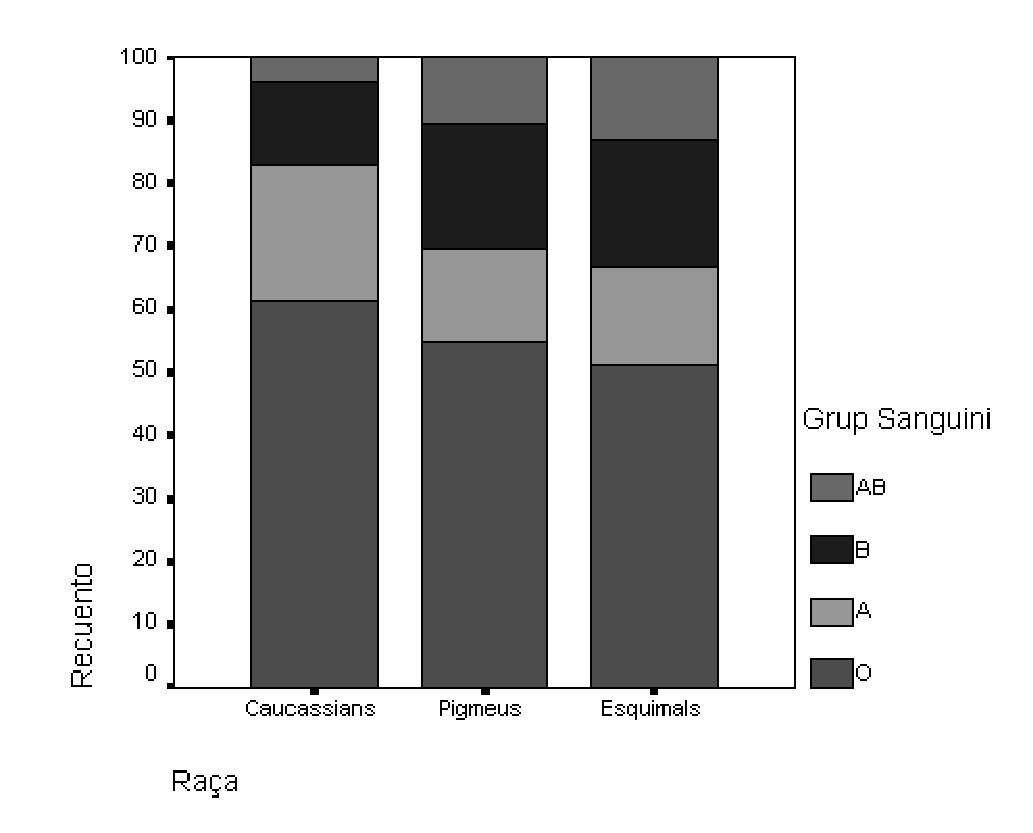
\includegraphics{./imatges/TestHomog.eps}
\end{center}
\caption{Diagrama de barres m\'{u}ltiples que mostra com es
distribueixen els grups sanguinis entre cada
ra\c{c}a}\label{testhomog}
\end{figure}
